\chapter{Comunicaciones}
\section{Pasarela de abordo}

El programa implementa una pasarela de comunicación entre la cámara Intel RealSense D435i y la estación de tierra. Su función 
principal es separar la información capturada por la cámara en distintos canales de comunicación: vídeo RGB transmitido mediante RTSP, 
datos inerciales enviados por UDP y datos de profundidad almacenados en un archivo \texttt{.bag} para su posterior análisis y validación.

La ejecución se organiza en varias tareas concurrentes. El hilo principal inicializa la configuración del sistema, lanza los hilos 
auxiliares y mantiene activo el servidor RTSP mediante el bucle principal de GStreamer. De forma paralela, un hilo supervisa la conexión 
de la cámara, otro adquiere los datos de la RealSense y un tercer hilo se encarga del envío periódico de la información inercial mediante 
UDP.


El flujo de ejecución comienza con la lectura de la configuración del sistema, donde se definen parámetros como el puerto RTSP, el punto 
de montaje, la resolución de imagen, la frecuencia de captura y el modo de depuración. En modo normal, el sistema espera a detectar la 
cámara física antes de iniciar la adquisición. En modo depuración, los datos se leen directamente desde un archivo \texttt{.bag}, lo que 
permite reproducir capturas previas sin necesidad de disponer de la cámara conectada.

Una vez iniciada la adquisición, cada paquete recibido desde la RealSense se clasifica según su tipo de flujo. Las muestras del giroscopio 
y del acelerómetro se escalan y almacenan en la estructura compartida \texttt{rs\_data}. Las imágenes RGB se encapsulan en buffers de 
GStreamer y se introducen en el elemento \texttt{appsrc}, desde donde son codificadas en H.264 y publicadas mediante RTSP. Por otro lado, 
el canal de profundidad se almacena en el archivo de registro para su posterior comparación con los resultados obtenidos por el algoritmo 
de navegación.

La comunicación con la estación de tierra se habilita mediante un mecanismo de conexión por UDP. Cuando el cliente envía un mensaje de 
establecimiento de conexión, el sistema almacena su dirección y activa el envío periódico de datos inerciales. Esta misma variable de 
estado también se utiliza para controlar el envío del flujo de vídeo, evitando introducir imágenes en el servidor RTSP cuando no existe 
ningún cliente conectado.

La arquitectura de funcionamiento se muestra en la Figura~\ref{fig:threads_comms}

\begin{figure}[H]
    \ffigbox[\FBwidth] {
        \caption[Arquitectura de funcionamiento de la pasarela.]{Arquitectura de funcionamiento de la pasarela.}
        \label{fig:threads_comms}
    }
    {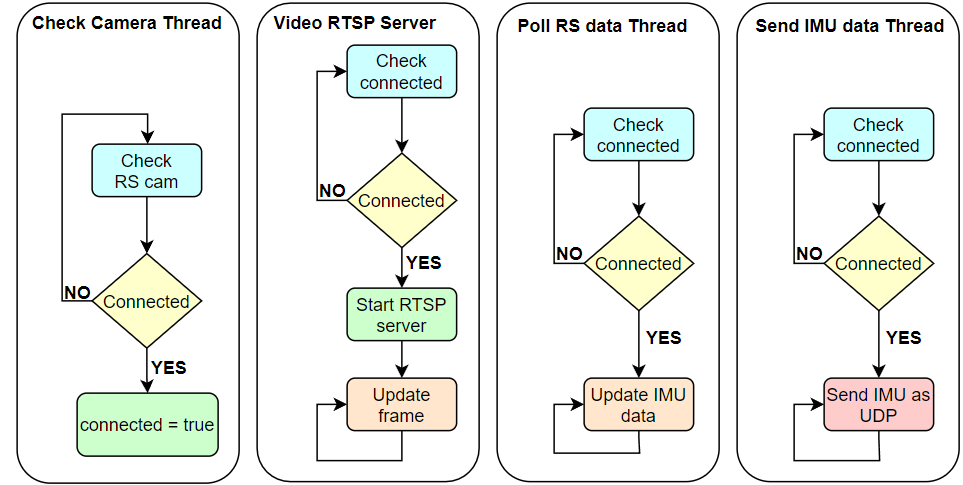
\includegraphics[scale=0.55]{images/threads_pasarela.png}}
\end{figure}


\section{Recepción de datos}

\subsection{Proceso de adquisición y sincronización de datos}

El módulo de adquisición se encarga de leer los datos procedentes de la Jetson Nano y generar paquetes de entrada 
sincronizados para el algoritmo de navegación. Cada paquete contiene una imagen RGB y un conjunto de muestras inerciales comprendidas 
entre dos imágenes consecutivas.

El proceso comienza en la incialización del receptor RTSP y la creación del socket UDP para la recepción de los 
datos inerciales.

Una vez inicializado el sistema, se lanza un hilo de adquisición. Este hilo se ejecuta interativamente. Las muestras 
inerciales se almacenan en un buffer independiente, uno para el acelerómetro y otro para el giróscopo. Cada muestra queda asociada a una 
marca temporal.

Cuando se recibe una imagen RGB válida, el algoritmo comprueba que existan suficientes muestras de IMU antes y después del instante de 
captura de la imagen. A continuación, se seleccionan los instantes de integración comprendidos entre la imagen anterior y la imagen actual. Para 
cada uno de estos instantes se interpolan las medidas del acelerómetro y del giróscopo, generando así una secuencia de muestras 
inerciales sincronizadas con el intervalo visual.


Finalmente, se construye un paquete, que contiene la imagen RGB y el conjunto de 
muestras IMU interpoladas. Este paquete se introduce en una cola de salida, desde donde puede ser 
consumido posteriormente por el algoritmo de navegación. Este proceso se muestra en la Figura~\ref{fig:frame_imu}.

\begin{figure}[H]
    \ffigbox[\FBwidth] {
        \caption[Esquema de adquisición de datos.]{Esquema de adquisición de datos.}
        \label{fig:frame_imu}
    }
    {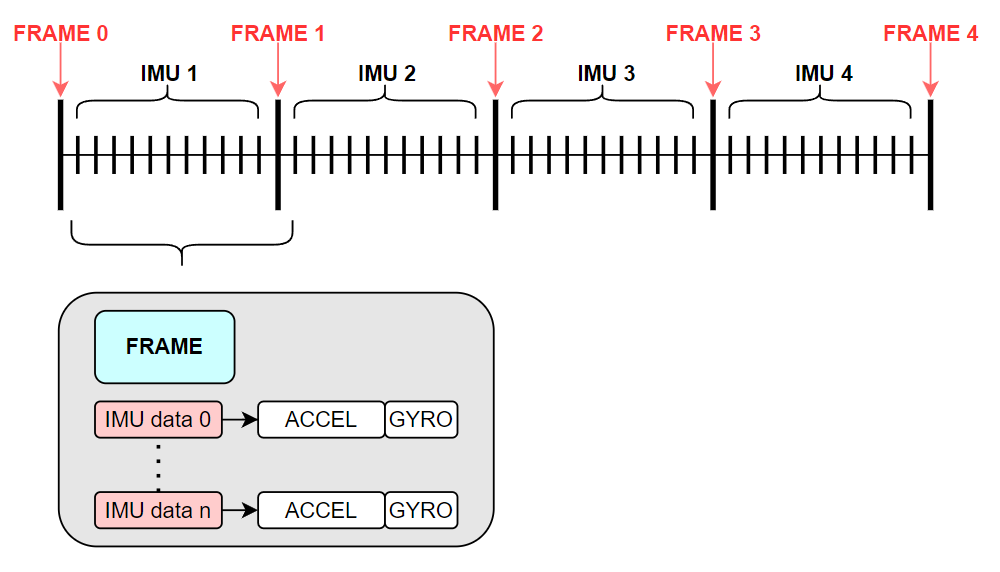
\includegraphics[scale=0.55]{images/frame_imu_arq.png}}
\end{figure}



\subsection{Interpolación de medidas inerciales}

Las medidas de la IMU se adquieren a frecuencias diferentes y no están necesariamente sincronizadas con los fotogramas 
visuales. Por ello, se realiza una interpolación lineal de las medidas inerciales, de forma que se obtenga una muestra de 
acelerómetro y giróscopo en los mismos instantes temporales. Además, se fuerza que la última muestra inercial del paquete 
coincida temporalmente con el fotograma visual correspondiente.

Sea un buffer de muestras inerciales definido como $\mathcal{B}$, donde cada muestra está formada por una marca 
temporal $t_i$ y una medida vectorial $\mathbf{v}_i \in \mathbb{R}^3$, correspondiente a una aceleración o a una velocidad 
angular:

\begin{equation}
\begin{aligned}
    \mathcal{B}&=\left\{\left(t_0, \mathbf{v}_0\right),\left(t_1, \mathbf{v}_1\right),\ldots,\left(t_N, \mathbf{v}_N\right)\right\},\\[2mm]\mathbf{v}_i&=
    \begin{bmatrix}
        v_{x,i} &
        v_{y,i} &
        v_{z,i}
    \end{bmatrix}^{T}.
\end{aligned}
\end{equation}

Para obtener el valor de la IMU en un instante $t$, el algoritmo busca dos muestras consecutivas que encierren dicho 
instante. Si $t$ queda fuera del intervalo temporal disponible, la interpolación se considera no válida:

\begin{equation}
\begin{aligned}
    t_i \leq t \leq t_{i+1},
    \qquad
    t \in \left[t_0,t_N\right].
\end{aligned}
\end{equation}

Una vez localizado el intervalo, se calcula el factor de interpolación lineal $\alpha$ y se obtiene la medida interpolada 
$\mathbf{v}(t)$ como combinación lineal entre las dos muestras consecutivas:

\begin{equation}
\begin{aligned}
    \Delta t_i
    &=
    t_{i+1}-t_i,
    \\[1mm]
    \alpha
    &=
    \frac{t-t_i}{\Delta t_i},
    \\[1mm]
    \mathbf{v}(t)
    &=
    \mathbf{v}_i
    +
    \alpha
    \left(
        \mathbf{v}_{i+1}
        -
        \mathbf{v}_i
    \right).
\end{aligned}
\label{eq:interpolacion_imu}
\end{equation}

De forma equivalente, la interpolación anterior puede expresarse por componentes como

\begin{equation}
    \mathbf{v}(t)
    =
    \begin{bmatrix}
        v_{x,i} + \alpha \left(v_{x,i+1} - v_{x,i}\right) \\
        v_{y,i} + \alpha \left(v_{y,i+1} - v_{y,i}\right) \\
        v_{z,i} + \alpha \left(v_{z,i+1} - v_{z,i}\right)
    \end{bmatrix}.
\end{equation}

En el caso particular en el que dos muestras consecutivas tengan prácticamente la misma marca temporal, se evita la 
división por un valor cercano a cero y se asigna directamente la primera muestra del intervalo:

\begin{equation}
    \mathbf{v}(t)
    =
    \begin{cases}
        \mathbf{v}_i
        &
        \text{si }
        \left|t_{i+1}-t_i\right| < 10^{-9},
        \\[1mm]
        \mathbf{v}_i
        +
        \alpha
        \left(
            \mathbf{v}_{i+1}
            -
            \mathbf{v}_i
        \right)
        &
        \text{en caso contrario}.
    \end{cases}
\end{equation}

Este procedimiento se aplica de forma independiente al acelerómetro y al giróscopo. Así, para cada instante $t_k$ se 
obtienen las medidas interpoladas

\begin{equation}
\begin{aligned}
    \mathbf{a}_k
    &=
    \mathbf{a}(t_k),
    &
    \boldsymbol{\omega}_k
    &=
    \boldsymbol{\omega}(t_k),
    \\[1mm]
    \Delta t_k
    &=
    t_k - t_{k-1}.
\end{aligned}
\end{equation}

Finalmente, cada muestra inercial generada para el paquete de navegación queda definida como

\begin{equation}
    \mathcal{I}_k
    =
    \left\{
        t_k,
        \Delta t_k,
        \mathbf{a}_k,
        \boldsymbol{\omega}_k
    \right\}.
\end{equation}
Un ejemplo de sincronización se muestra en la Figura~\ref{fig:sinc_source_man}.

\begin{figure}[H]
    \ffigbox[\FBwidth] {
        \caption[Ejemplo de sincronización de datos.]{Ejemplo de sincronización de datos.}
        \label{fig:sinc_source_man}
    }
    {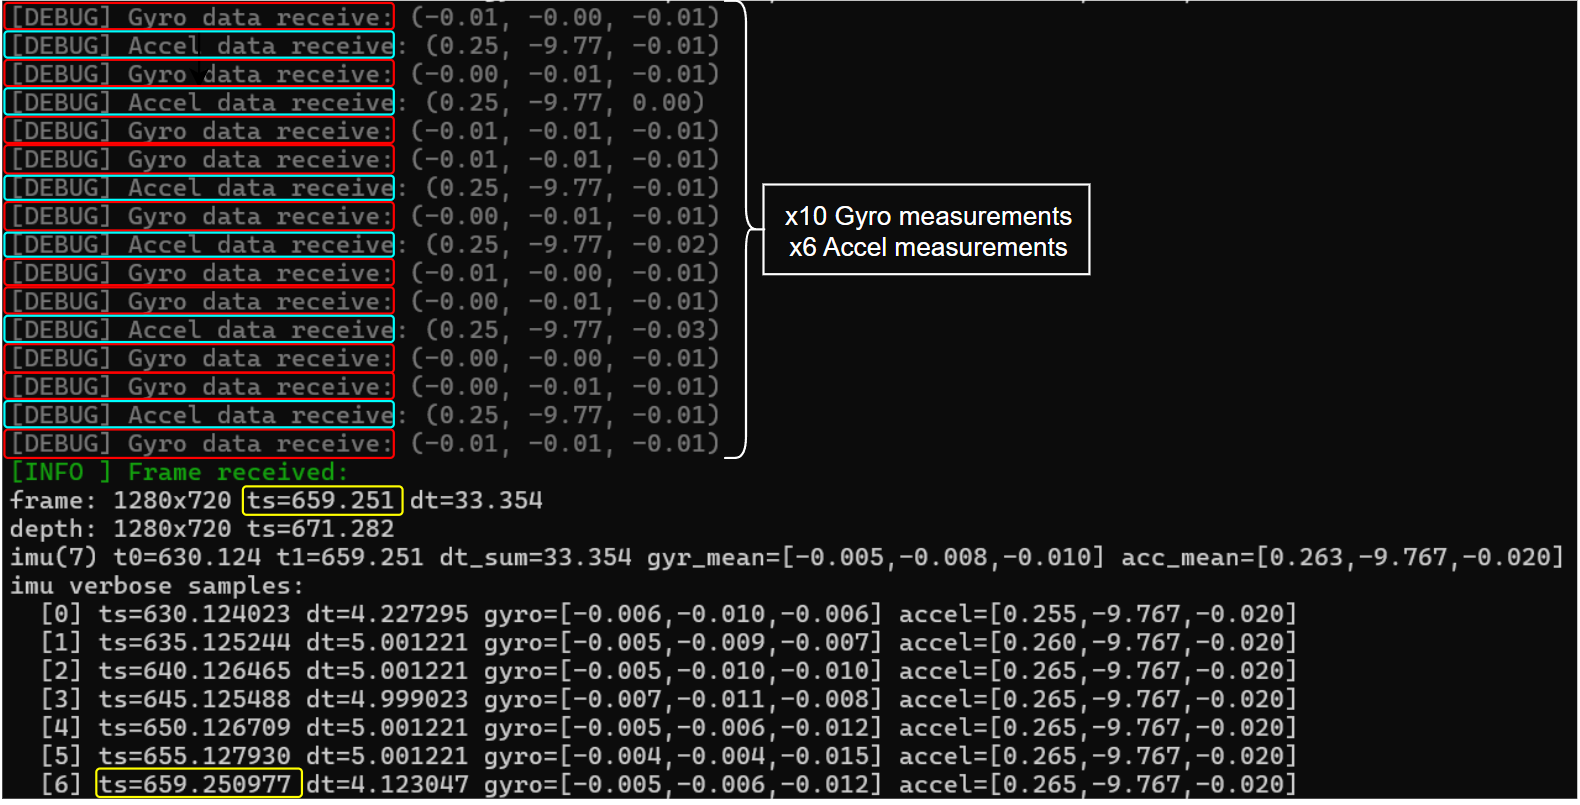
\includegraphics[scale=0.3]{images/source_manager_sync.png}}
\end{figure}

\section{Envío de comandos de velocidad}

Una vez calculado el comando de velocidad por el controlador, este debe enviarse al UAV para su ejecución. Dicho comando 
está compuesto por una velocidad lineal y una velocidad angular, expresadas en el sistema de referencia empleado por el 
algoritmo de navegación:

\begin{equation}
    \mathbf{u}
    =
    \begin{bmatrix}
        v_x &
        v_y &
        v_z &
        \omega_z
    \end{bmatrix}^{T},
\end{equation}

donde $v_x$, $v_y$ y $v_z$ representan las componentes de velocidad lineal, y $\omega_z$ corresponde a la velocidad angular 
alrededor del eje vertical del UAV.

El envío de comandos se realiza desde la estación de tierra hacia la plataforma aérea mediante comunicación UDP. Esta 
solución permite transmitir consignas de control con baja latencia, lo cual resulta fundamental en aplicaciones de 
navegación autónoma. En la plataforma aérea, la Jetson Nano recibe estos comandos, los interpreta y los reenvía al 
controlador de vuelo para que sean ejecutados por el UAV.

Para evitar comportamientos bruscos o no deseados, antes del envío se aplican límites máximos a las componentes de 
velocidad. Esta saturación puede expresarse como

\begin{equation}
\begin{aligned}
    \bar{v}_i
    &=
    \operatorname{sat}
    \left(
        v_i,
        v_{i,\max}
    \right)
    =
    \max
    \left(
        -v_{i,\max},
        \min
        \left(
            v_i,
            v_{i,\max}
        \right)
    \right),
    \qquad
    i \in \{x,y,z\},
    \\[2mm]
    \bar{\omega}_z
    &=
    \operatorname{sat}
    \left(
        \omega_z,
        \omega_{z,\max}
    \right)
    =
    \max
    \left(
        -\omega_{z,\max},
        \min
        \left(
            \omega_z,
            \omega_{z,\max}
        \right)
    \right).
\end{aligned}
\end{equation}

Por tanto, el comando finalmente enviado al UAV queda definido como

\begin{equation}
    \bar{\mathbf{u}}
    =
    \begin{bmatrix}
        \bar{v}_x &
        \bar{v}_y &
        \bar{v}_z &
        \bar{\omega}_z
    \end{bmatrix}^{T}.
\end{equation}

De esta forma, el sistema garantiza que las consignas enviadas al UAV se mantienen dentro de los límites dinámicos 
definidos para la plataforma. 